\begin{figure}[h]
\centering
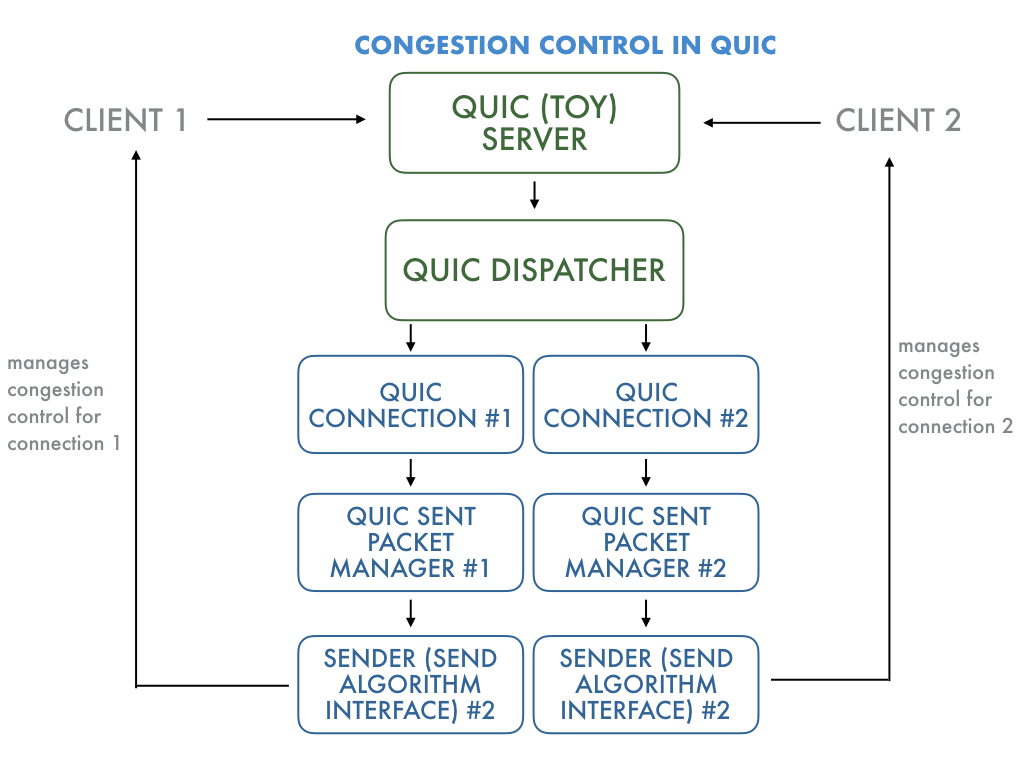
\includegraphics[scale=.45]{implementation/quiccc}
\caption{In QUIC, when the toy server sees a client request, the \ct{SimpleDispatcher} object spawns a new \ct{QuicConnection} object that handles the connection. To manage sending packets, the \ct{QuicConnection} object creates a \ct{QuicSentPacketManager}. The \ct{QuicSentPacketManager} creates a \ct{Sender} object that uses the function callbacks from the \ct{SendAlgorithmInterface} specified as the current congestion control setting.}
\label{fig:quiccc_diagram}
\end{figure}
